% vim: ts=4 sts=4 sw=4
\documentclass[portuguese, a4paper]{article}
\usepackage[T1]{fontenc}
\usepackage[utf8]{inputenc}
\usepackage{babel}
\usepackage[margin=2.5cm]{geometry}
\usepackage{lmodern}

\usepackage{graphicx}
\graphicspath{{imagens/}}
\usepackage{wrapfig,lipsum}
\usepackage{bold-extra}
\usepackage{epstopdf}
\usepackage{float}
\usepackage{scalerel}
\usepackage{enumerate}
\usepackage{indentfirst}
\usepackage{mathtools}
\usepackage{amsmath}
\allowdisplaybreaks
\usepackage{amssymb}
\usepackage{listings}
\usepackage{color}
\usepackage{textcomp}
\usepackage{caption}
\usepackage{hyperref}
\hypersetup{colorlinks,
			citecolor=black,
			filecolor=black,
			linkcolor=black,
			urlcolor=blue}
\newcommand\showdiv[1]{\overline{\smash{\hstretch{.5}{)}\mkern-3.2mu\hstretch{.5}{)}}#1}}
\newcommand\ph[1]{\textcolor{white}{#1}}
\newcommand\tu[0]{\textunderscore}
\newcommand\eq[0]{\Leftrightarrow}

\definecolor{dkgreen}{rgb}{0,0.6,0}
\definecolor{gray}{rgb}{0.5,0.5,0.5}
\definecolor{mauve}{rgb}{0.58,0,0.82}
\definecolor{mygreen}{RGB}{28,172,0} % color values Red, Green, Blue
\definecolor{mylilas}{RGB}{170,55,241}


\lstset{frame=tb,
  language=Octave,
  aboveskip=3mm,
  belowskip=3mm,
  showstringspaces=false,
  columns=flexible,
  basicstyle={\small\ttfamily},
  numbers=none,
  numberstyle=\tiny\color{gray},
  keywordstyle=\color{blue},
  commentstyle=\color{dkgreen},
  stringstyle=\color{mauve},
  breaklines=true,
  breakatwhitespace=true,
  tabsize=3,
  extendedchars=true,
  literate=	{á}{{\'a}}1	{ã}{{\~a}}1	{â}{\^{a}}1	{é}{\'{e}}1	{ç}{\c{c}}1
  			{ã}{\~{a}}1	{à}{\`{a}}1 {ê}{\^{e}}1 {í}{\'{i}}1	{ó}{\'{o}}1
			{õ}{\~{o}}1 {ô}{\^{o}}1	{ú}{\'{u}}1 {Ç}{\c{C}}1 {É}{\'{E}}1,
}

% ----- Cabeçalho e rodapé -----
\usepackage{fancyhdr}
\pagestyle{fancy}
\fancyhf{}

\renewcommand{\headrulewidth}{1pt}
\renewcommand{\footrulewidth}{0.5pt}

\rhead{2º Trabalho Computacional}
\lhead{Matemática Computacional}
\rfoot{Página \thepage}
\lfoot{\small Engenharia Eletrotécnica e de Computadores - IST}

\usepackage{pdfpages}

%center sections
%http://tex.stackexchange.com/a/107282
\usepackage{sectsty}
\sectionfont{\centering}

\begin{document}
\includepdf[pages={1}]{capa/capa.pdf}

% Secções em números romanos.
\renewcommand{\thesection}{\Roman{section}}
\renewcommand{\thesubsection}{\arabic{subsection}.}
% Subsubsecções no estilo a), b), ...
\renewcommand{\thesubsubsection}{\alph{subsubsection})}

\renewcommand{\contentsname}{Índice}
\tableofcontents
\newpage

\section{} \label{sec:I}
	\par
	Todos os ficheiros de código encontram-se em anexo no final deste relatório. Os mesmos devem ser corridos no programa \emph{Octave}.

	\subsection{} \label{sec:I.1}
	\par
	Resposta no ficheiro \texttt{I/min\tu quad.m}, corrido pelo \emph{script} \texttt{I/1.m}, onde é possível alterar os pontos tabelados, os respetivos pesos e as funções de base.

	\subsection{} \label{sec:I.2}
	\par
	Para os dados tabelados:
	\begin{table}[H]
		\centering
		\begin{tabular}{c|c|c|c|c|c|c|c|c|c|c}
			\hline
			$1/e$	& 0.345	& 0.287	& 0.251	& 0.225	& 0.207	& 0.186	& 0.161	& 0.132	& 0.084	& 0.060	\\ \hline
			$s$		& 367	& 311	& 295	& 268	& 253	& 239	& 220	& 213	& 193	& 192	\\ \hline
			$d$		& 17	& 9		& 9		& 7		& 7		& 6		& 6		& 6		& 5		& 5		\\ \hline
		\end{tabular}
		\caption{Dados tabelados.}
	\end{table}

	\par
	Foram obtidas as três funções aproximadoras pedidas, através da função desenvolvida em \ref{sec:I.1}, pelos ficheiros \texttt{I/2\tu i.m}, \texttt{I/2\tu ii.m} e \texttt{I/2\tu iii.m}. Estes três ficheiros são corridos no \emph{script} \texttt{I/2.m}, onde as três funções aproximadoras resultantes são aplicadas aos pontos tabelados e são ainda desenhados os gráficos resultantes, assim como os pontos tabelados.

	\begin{figure}[H]
		\centering
		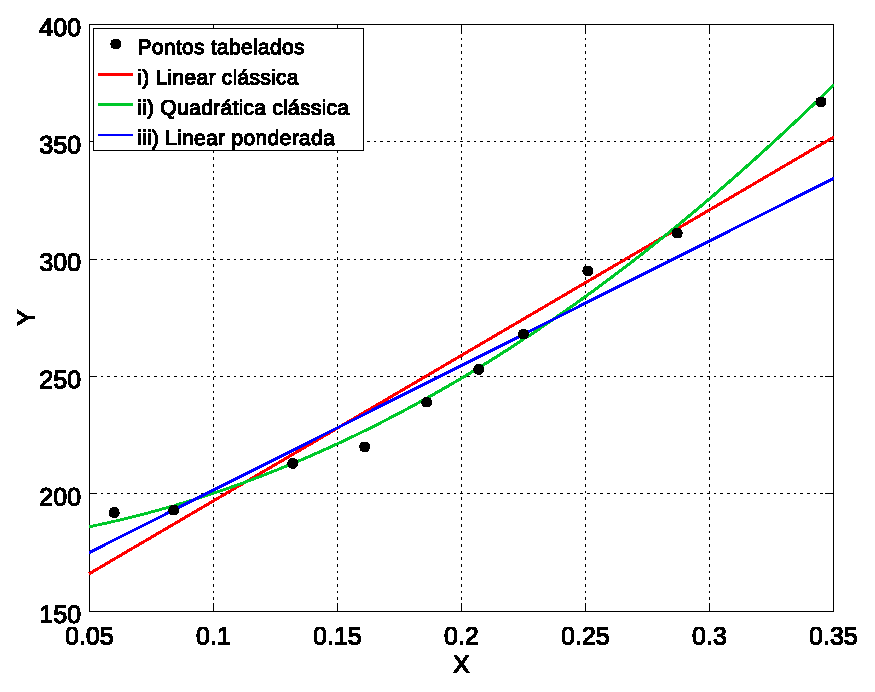
\includegraphics[width=0.80\linewidth]{I_fino}
		\captionsetup{width=0.80\linewidth}
		\caption{Diferentes funções aproximadoras dos pontos tabelados, pelos critérios dos mínimos quadrados clássico e ponderado.}
	\end{figure}

\newpage
\section{} \label{sec:II}
	\subsection{} \label{sec:II.1}
	\par
	Resposta no ficheiro \texttt{II/simpson.m}, corrido pelo \emph{script} \texttt{II/1.m}, onde é possível alterar o intervalo de integração, o número de subintervalos e a função a integrar.

	\subsection{} \label{sec:II.2}
	\subsubsection{} \label{sec:II.2a)}
	\par
	Correndo o programa \texttt{II/2.m}, obtém-se:
	$$F =  1480.56848008215$$

	\subsubsection{} \label{sec:II.2b)}
	\par
	Correndo o programa \texttt{II/2.m}, obtém-se:
	\begin{table}[H]
		\centering
		\begin{tabular}{|c|c|c|c|}
			\hline
			$n$	& $S_n$				& $|F - S_n|$		& $\frac{|F - S_n/2|}{|F - S_n|}$ \\ \hline
			2	& 1219.63999486000	& 260.92848522216	& -					\\ \hline
			4	& 1426.86928844946	& 53.69919163269	& 4.85907659480		\\ \hline
			8	& 1473.14779849473	& 7.42068158743		& 7.23642309672		\\ \hline
			16	& 1479.85678890922	& 0.71169117293		& 10.42682819413	\\ \hline
			32	& 1480.51545319880	& 0.05302688335		& 13.42132759730	\\ \hline
			64	& 1480.56497529815	& 0.00350478401		& 15.12985771736	\\ \hline
			128	& 1480.56825767195	& 0.00022241020		& 15.75819799559	\\ \hline
			256	& 1480.56846613061	& 0.00001395154		& 15.94162455869	\\ \hline
			512	& 1480.56847921284	& 0.00000086931		& 16.04897985126	\\ \hline
		\end{tabular}
		\caption{Comparação dos erros da regra de Simpson para vários valores de N.}
		\label{tab:simp}
	\end{table}
	\par
	O erro da fórmula de Simpson composta com $N$ subintervalos é dado por:
	$$E_N^S(f) = -\frac{(b - a)h^4}{180}f^{(4)}(\xi), \xi \in [a,b]$$

	\par
	Dividindo $E_{N/2}^S(f)$ por $E_N^S(f)$ e como $h = \frac{(b - a)}{N}$, obtém-se:

	% > muh explicit
	% > muh TeX
	$$\frac{E_{N/2}^S(f)}{E_N^S(f)} =
	\frac{\frac{(b - a)}{180}\frac{(b - a)^4}{(\frac{N}{2})^4}f^{(4)}(\xi)}
		 {\frac{(b - a)}{180}\frac{(b - a)^4}{N^4}f^{(4)}(\xi)} =
	\frac{\frac{(b - a)^5}{180}\frac{1}{(\frac{N}{2})^4}f^{(4)}(\xi)}
		 {\frac{(b - a)^5}{180}\frac{1}{N^4}f^{(4)}(\xi)} =
	\frac{\frac{1}{\frac{N^4}{16}}}{\frac{1}{N^4}} = \frac{N^4}{\frac{N^4}{16}} =
	16\frac{N^4}{N^4} = 16$$

	\par
	Assim, teoricamente, esperamos que quando se duplica o número de subintervalos, o erro da fórmula de Simpson composta caia 16 vezes. Tal é verificado pela quarta coluna da Tabela \ref{tab:simp} quando $N$ tende para infinito ou, na prática, para um número suficientemente grande para garantir uma boa aproximação pela regra de Simpson. O rácio não é sempre igual a 16 por causa das primeiras aproximações para $N$ pequenos serem demasiado grosseiras.

\newpage
\section{} \label{sec:III}
	\subsection{} \label{sec:III.1}
	\par
	O programa desenvolvido tem o nome de \texttt{III/ponto\tu medio.m}. Recebe um intervalo
	$[a,b]$, uma função $f$ desenvolvida à parte, específica para cada problema de valor inicial,
	uma condição inicial $ y_\alpha $ e um número $n$ de subintervalos.

	\subsection{} \label{sec:III.2}
		\subsubsection{} \label{sec:III.2a)}
		\par
		Dividindo $\frac{dI}{dt}$ por $\frac{dS}{dt}$, obtemos:

		% completar as Equações
		\begin{equation}
		\begin{split}
			& \frac{dI}{dS} = -1 + \frac{300}{S} \Leftrightarrow \\
			& dI = \left(-1 + \frac{300}{S}\right)dS \Leftrightarrow \\
			& \int dI = \int\left(-1 + \frac{300}{S}\right)dS \Leftrightarrow \\
			& I = -S + 300ln~S + c
		\end{split}
		\end{equation}

		\par
		Para chegar ao valor de c, impõem-se as condições iniciais $I(0) = 1$ e $S(0) = 799$:

		\begin{equation}
		\begin{split}
			& I(0) = -S(0) + 300 \times ln(S(0)) + c \eq \\
			& c = -799 + 300ln(799) - 1 \eq \\
			& c \approx -1205.008
		\end{split}
		\end{equation}

		\par
		O número máximo de crianças doentes num dado momento pode ser obtido
		atráves do máximo de $I(S)$.
		\begin{equation}
			\label{eq:root}
			\frac{dI}{dS} = 0 \eq -1 + \frac{300}{S} = 0
			\eq S = 300
		\end{equation}

		\begin{equation}
		\begin{split}
			\label{eq:comp}
			 -1 + \frac{300}{S} > 0 \eq S < 300 \\
			 -1 + \frac{300}{S} < 0 \eq S > 300
		\end{split}
		\end{equation}

		\par
		A derivada de $I(S)$ tem um único zero em $S = 300$ \eqref{eq:root},
		e, como é maior que 0 para valores inferiores a 300 e menor que 0
		para valores superiores a 300 \eqref{eq:comp}, $I(S)$ tem um máximo
		em $S = 300$ que corresponde ao número de crianças suscetíveis
		quando o número de crianças infetadas é máximo.

		\par
		Substituindo na equação, obtemos:
		\begin{equation}
			I(300) = -300 + 300 \times ln(300) - 1205.008 \approx 206
		\end{equation}

		\subsubsection{} \label{sec:III.2b)}
		\par
		Em primeiro lugar, verifiquemos que o valor de $S$ para o qual $I(S) = 0$ é menor que 200.

		\par
		Como demonstrado em \eqref{eq:comp}, no intervalo
		$[-\infty,300[~\setminus\{0\}$ a função $\frac{dI}{dS}$ é diferente de
		zero. Como $]0,200] \subset [-\infty,300]~\setminus\{0\}$, também nesse
		intervalo a função $\frac{dI}{dt}$ é diferente de zero. Nestas condições
		o Teorema de Rolle garante que no intervalo $]0,200]$ existirá no máximo
		uma raiz da função $I(S)$.

		\par
		Como $I(1) < 0$ e $I(200) > 0$ pelo Teorema de Bolzano garantimos a
		existência de pelo menos uma raiz de $I(S)$ nesse intervalo.

		\par
		Pelas duas conclusões anteriores podemos deduzir a existência e
		unicidade da raiz de $I(S)$ no intervalo $]0, 200]$.

		\par \null \par
		O fim da epidemia corresponde corresponde à raiz da função $I$ cuja
		existência acabamos de provar. Essa raiz será igual ao número de
		crianças não afetadas pela epidemia. Para encontrar essa raiz iremos
		interpolar a função inversa de $I$.

		\begin{equation}
			I(S) = 0 \rightarrow S = I^{-1}(0)
		\end{equation}

		\par
		O seu cálculo pode ser simplificado pela utilização da função
		\texttt{polyfit} do Octave.  Assim, escrevemos um pequeno script em
		Octave que permite rapidamente encontrar a raiz da função $I$
		utilizando a sua inversa. Esse script pode ser encontrado em
		\texttt{III/III\tu b.m}. \footnote{Instruções de utilização podem ser
		encontradas no código fonte.}

		\par
		A execução do script \texttt{III/III\tu b.m} para o intervalo $[1, 200]$
		com 1000 intervalos de interpolação para um polinómio de grau 3 devolve
		um valor da raiz $z \approx 73.899$.

		%Se a epidemia acabar quando o número de crianças infetadas for 0,
		%então, teremos que ver quantas crianças estão suscetíveis neste ponto,
		%pois essas nunca serão infetadas, pelo menos nesta epidemia.
		%Especialmente por ser varicela, uma doença que só se costuma ter uma
		%vez, podemos ver que a transição de estados de uma criança é otimamente
		%descrita por este diagrama.
		%%lembras-te daquele diagrama de estados?...consegues?xD

		%Uma criança, tirando a paciente zero, começa no estado suscetível. Passa
		%para o estado infetado quando é infetada e depois de recuperada fica no estado de recuperada até ao fim da
		%epidemia e provavelmente até ao fim da sua vida.

		%%se não conseguires ou não te apetecer, é só preciso trocar algumas palavras

		%Podia-se ter usado uma função que interpola polinómios já implementada.
		%Em vez disso conseguímos um resultado igualmente satisfatório através de funções criadas por nós, pois
		%quando o grupo foi avisado da existência e possibilidade de utilização de funções como $polynomial$ %era assim que se chamava, não era?
		%já tinha tudo implementado.

		%%consegues por + bonito:
        %% o que é que é suposto ser o \^ ?
		%Quer-se um S tal que $I(S) = 0 \rightarrow S = I^{-1}(0)$.
		%A interpolação inversa consiste em aproximar a função inversa através de polinómios.
		%Ao fazer-se isto, espera-se depois conseguir encontrar uma aproximação
		%para a imagem de $I^{-1}(0)$,
		%que será o S que nós procuramos.
		%\par
		%Depois de utilizarmos as duas funções, concluímos que $I^{-1}(0) = 70$.

		\subsubsection{} \label{sec:III.2c)}
		\par
		Utilizando a expressão $I(t) = -S(t) + 300ln~S(t) + c$ e substituindo
		os $I$ pelo lado direito da equação, obteremos uma equação na forma de
		um PVI\@. A partir daí podemos usar o método do ponto médio\footnote{A
		implementação pode ser encontrada em \texttt{III/ponto\tu medio.m}}
		para calcular aproximações $y_0$, $y_1$, \ldots, $y_N$ dos pontos $x_0
		= 0$, $x_1 = h$, \ldots, $x_N = nh$ e desenhar o gráfico de acordo
		com esses pontos.

		\par
		Para obtermos um gráfico para o número de pessoas infetadas ao longo do
		tempo, usamos os nossos pontos já cálculados. Como $I$ pode ser escrito
		em função de $S$, $I(x_i) = -S(x_i) + 300ln~S(x_i) - 1205$.

		\par
		Assim, para cada momento podemos saber uma aproximação do número de
		pessoas infetadas, obtendo-se assim	o gráfico da função I(t).

		\par \null \par
		Finalmente, para se conseguir o gráfico de $R$ foi necessário
		dividir $\frac{dR}{dt}$ por $\frac{dS}{dt}$ e integrar:

		\begin{equation}
		\begin{split}
			\frac{\frac{dR}{dt}}{\frac{dS}{dt}} = \frac{0.3 I}{-0.0001 S I}
			\eq
			\frac{dR}{dS} = &-\frac{300}{s} \eq dR =
			-\frac{300}{s} dS
			\int \frac{dR}{dt}dt = \int -\frac{300}{s} \frac{dS}{dt}dt
			\eq \\ \newline
			& R(t) = -300 ln(S(t)) + c
		\end{split}
		\end{equation}

		\begin{equation}
			0 = -300 ln(799) + c \eq \\
			c = 2005.008 \\
		\end{equation}

		\begin{equation}
			R(t) = -300\, ln(S(t)) + 2005.008
		\end{equation}

		\par
		Ficamos com uma relação entre $R(t)$ e $S(t)$. Como temos uma
		aproximação para $S(t)$, é suficiente substituir as aproximações na
		expressão obtida e, assim, obter uma aproximação para $R(t)$.

		\par
		Juntando os três gráficos:

		\begin{figure}[H]
			\centering
			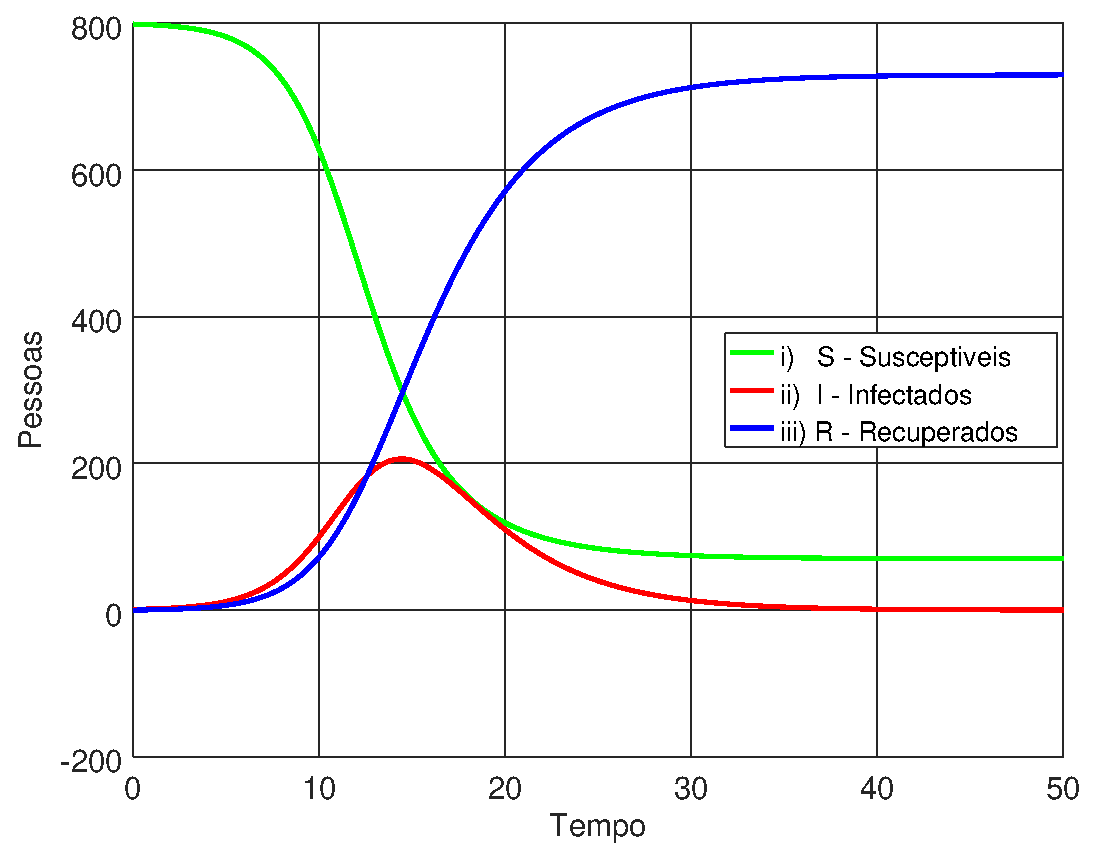
\includegraphics[width=0.70\linewidth]{IIIc_fitted}
			\captionsetup{width=0.70\linewidth}
			\caption[Caption]{Evolução das variáveis $S$, $I$, $R$ ao longo do
			tempo.
			\footnotemark}
		\end{figure}
		\footnotetext{O	código utilizado para gerar o gráfico pode ser
		encontrado no ficheiro \texttt{III/c.m} em anexo.}

		\par
		Relacionando o gráfico com o problema em questão, notamos que as aproximações feitas devem estar
		bastante próximas do valor certo/real de cada função, pois os gráficos comportaram-se como esperado e cumpriram as respetivas propriedades.

		%estou só a experimentar este itemize
		\begin{itemize}
		\item Como o limite superior de pessoas da amostra é 800, nenhuma função tem uma imagem acima de 800.
		\item O valor máximo para o número de pessoas infetadas num dado momento é 206 e tal pode-se confirmar pelo gráfico.
		\item Foi visto na alínea b) que o número de pessoas
		nunca infetadas é algo perto de 70. % TODO: verificar que é 70 certo ou nao...
		No gráfico, pode observar-se que quando $I(t) = 0$, $S(t) \approx 74$ e que fica constante nesse valor a partir do instante em que $I(t) = 0$.
		Faz todo o sentido ser constante a partir desse momento, porque quando
		se recupera a última pessoa infetada, deixa de ser possivel contrair
		varicela e a partir daí o número de pessoas suscetíveis, isto é, que
		nunca contrairam varicela, não se altera.
		\item Em termos de interpretação do problema, o formato do gráfico da função das pessoas recuperadas assenta nas interpretações
		feitas sobre o problema. Se deixam de haver infetados a partir de determinado momento,
		também a partir desse momento o número de recuperados não se irá
		alterar.
		\end{itemize}

\newpage
\section{Anexos}
\subsection{I}
	\texttt{I/min\tu quad.m}
	\lstinputlisting{../src/I/min_quad.m}

	\texttt{I/1.m}
	\lstinputlisting{../src/I/1.m}

	\texttt{I/2\tu i.m}
	\lstinputlisting{../src/I/2_i.m}

	\texttt{I/2\tu ii.m}
	\lstinputlisting{../src/I/2_ii.m}

	\texttt{I/2\tu iii.m}
	\lstinputlisting{../src/I/2_iii.m}

	\texttt{I/2.m}
	\lstinputlisting{../src/I/2.m}

\newpage
\subsection{II}
	\texttt{II/simpson.m}
	\lstinputlisting{../src/II/simpson.m}

	\texttt{II/1.m}
	\lstinputlisting{../src/II/1.m}

	\texttt{II/2.m}
	\lstinputlisting{../src/II/2.m}

\newpage
\subsection{III}
	\texttt{III/c.m}
	\lstinputlisting{../src/III/c.m}

	\texttt{III/III\tu b.m}
	\lstinputlisting{../src/III/III_b.m}

	\texttt{III/ponto\tu medio.m}
	\lstinputlisting{../src/III/ponto_medio.m}

	\texttt{III/f.m}
	\lstinputlisting{../src/III/f.m}

\end{document}
